Many approaches may be considered while setting $\vecnot{\alpha},\vecnot{\beta}$ in order to achieve optimal utilization of the spatial IIR structure in (\ref{eqn:GeneralFeedbackTransferFunction}), all sharing the same purpose of minimizing the IIR component (i.e. the denominator) for specific spatially selected signals.
One naturally considered approach is the dual-conventional-beamformer (DCBF). In this approach, to achieve minimization of the IIR component,$ \vecnot{\beta}^{T}\vecnot{d}_{\theta_{s}}e^{-j\omega\tau_{s}} = 4c^{2}\tau_{s}^{2} $ (where $\tau_{s}$ is determined by the target's location), in order to achieve the desired high spatial selectivity. Considering the array phase and gain mismatch, we present $\rho = re^{\Phi}$, which will function as the array-mismatch-factor. Combined with the conventional beamformer (\cite{VanTrees2002DetectionIV}) we set $ \vecnot{\alpha} = \frac{1}{4c^{2}\tau_{s}^{2}}\vecnot{\beta} = \frac{\rho}{N}\vecnot{d^{*}_{s}e^{-j\tau_{s}}} $). Comparing the perfectly-aligned scenario $\left(\theta = \theta_{s}, \tau = \tau_{s}\right)$ with the general scenario, enables calculation of the half-power-beamwidth (HPBW) by setting $\left|\frac{H_{\theta_{s}\tau_{s}}\left(\omega{}\right)}{H_{\theta,\tau}\left(\omega{}\right)}\right|^{2} = 2$, which translates to 
\begin{align}
\label{eqn_arrPerformance_beamwidth_3dB}
\Hr{\theta}{\tau}{}
\triangleq
\fbBpRatio
=
2\ .
\end{align}
\ifdefined\DEFIncludeAttenuation
    Following \cite{VanTrees2002DetectionIV}'s steps (discussed in section \ref{section_arrayPerformance_classicULA}), we investigate $\Hr{\theta}{\tau}{}$ through calculation of its multivariate (i.e. $\dTheta\triangleq\theta-\theta_{s}, \dTau\triangleq\tau-\tau_{s}$) Taylor series. Considering the perfect phase alignment scenario (i.e. $\dTau=0$), as shown in (Figure \ref{fig_feedbackULA_beamwidth_Nx_HPBW_1_r_2}), one can observe that $\frac{N\dTheta_{HPBW}}{\left(1-r\right)^{2}}$ tends to an $r$-dependent finite limit when $N$ increases. 
    \begin{figure}
        \label{fig_feedbackULA_beamwidth_Nx_HPBW_1_r_2}
        \centering
        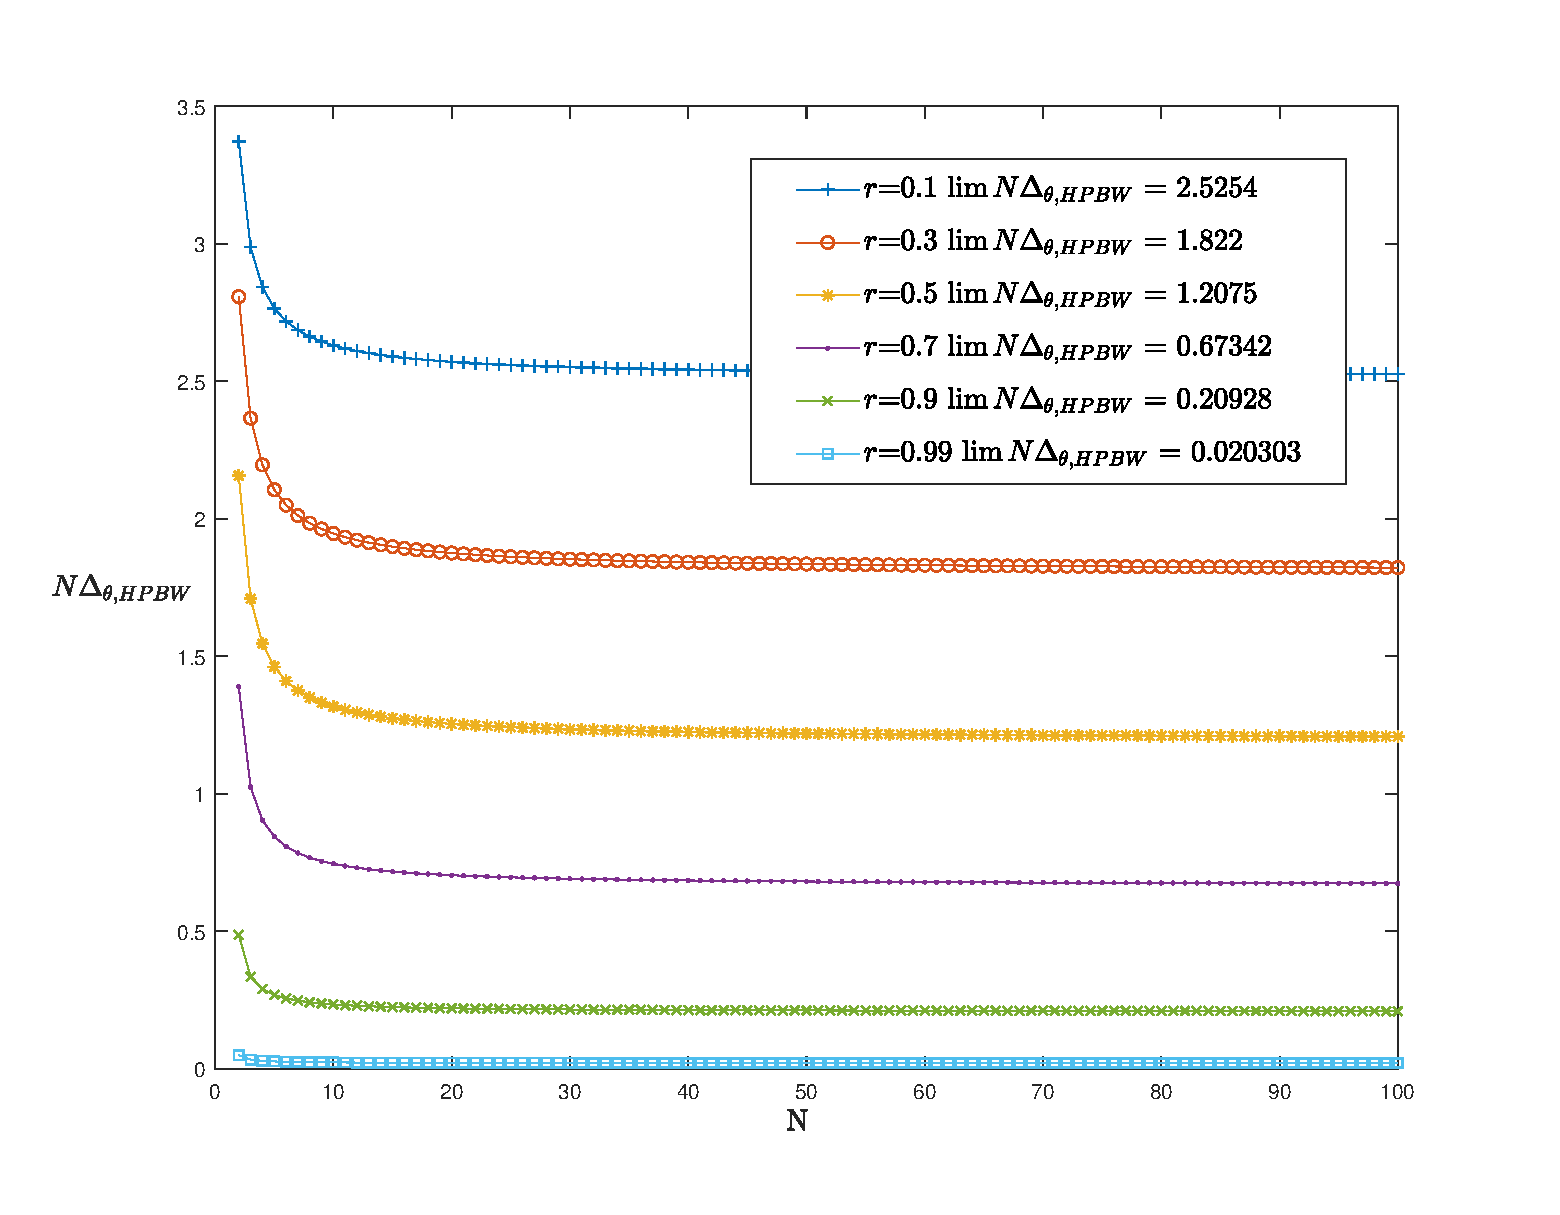
\includegraphics[width=0.8\linewidth]{./Media/spatial_IIR_MATLAB/beamwidth/HPBW_vs_N_various_r.eps}
        \caption{Plot of $N\dTheta_{HPBW}$ vs. N for various $r$ values. In each simulation, $r$ is constant and $\dTheta_{HPBW}$ is calculated for each $N$ separately and the stored value is $N\dTheta_{HPBW}$.}
    \end{figure}
    Plotting the limits of $\frac{N\dTheta_{HPBW}}{\left(1-r\right)^{2}}$ as a function of $r$, as can be seen in (Figure \ref{fig_feedbackULA_beamwidth_limit_r_dependent}), reveals that the limit is determined by $\frac{2}{1-r}$.
    \begin{figure}
        \label{fig_feedbackULA_beamwidth_limit_r_dependent}
        \centering
        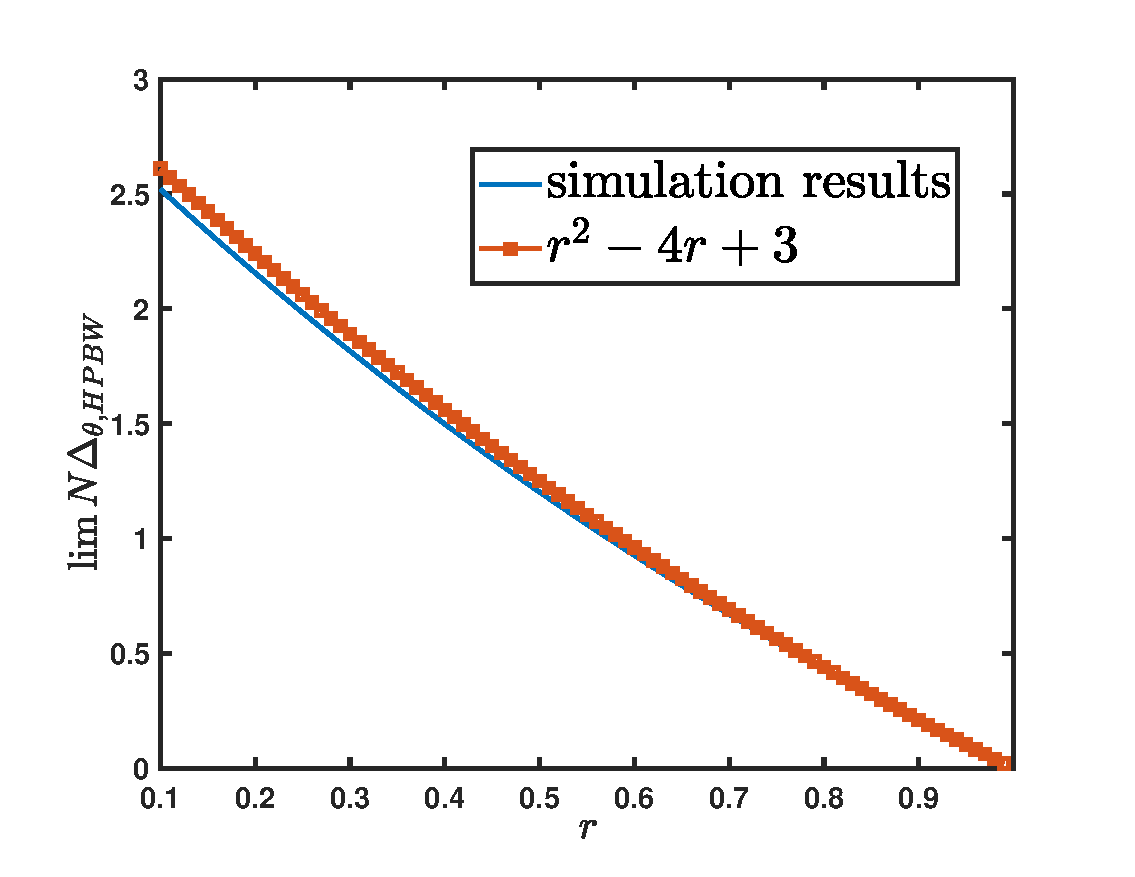
\includegraphics[width=0.8\linewidth]{./Media/spatial_IIR_MATLAB/beamwidth/HPBW_limit_vs_r.eps}
        \caption{Plot of $\underset{N\to\infty}{lim}N\dTheta_{HPBW}$ vs. $r$ and comparing to $r^{2}-4r+3$}
    \end{figure}
    These two important empirical observations allows us the formulation of the feedback based HPBW expression
    \begin{equation}
            \dTheta_{HPBW} =& \frac{\left(r-1\right)\left(r-3\right)}{N}
    \end{equation}
    which is naturally compared of the known \cite{VanTrees2002DetectionIV} matching passive ULA case (i.e. $\frac{\pi{}Nd}{\lambda}u = 1.4$, where $u\triangleq{}2\cos\left(\theta_{g}\right)$) and translated to the DCBF feedback related HPBW improvement factor ($\triangleq\mu_{DCBF}$)
    \begin{equation}
        \mu_{DCBF}=\frac{1.4}{\left(r-1\right)\left(r-3\right)},
    \end{equation}
    stating that a perfectly aligned array (i.e. $r\to1$) will achieve a zero-width spatial beam.
    % Using L'Hôpital's rule (due to $\frac{0}{0}$ expressions when setting $\dTheta=0$), we express its $4^{th}$ series
    % \begin{equation}
    %     \label{eqn_FIMelements}
    %     \begin{split}
    %         \evalat{\Hr{\theta}{\tau}{}}{\dTheta\to{}0,\dTau\to{}0} \approx& 1
    %         \\&
    %         +\frac{1}{1!}\binom{1}{0}0\dTheta
    %         \\&
    %         +\frac{1}{1!}\binom{1}{1}\frac{4r}{\tau_{s}(r-1)}\dTau
    %         \\&
    %         +\frac{1}{2!}\binom{2}{0}\frac{\left(N-1\right)\left(n-4r+2Nr+1\right)}{6\left(r-1\right)^{2}}\dTheta^{2}
    %         \\&
    %         +\frac{1}{2!}\binom{2}{1}\frac{-r\omega\left(N-1\right)}{\left(r-1\right)^{2}}\dTheta\dTau
    %         \\&
    %         +\frac{1}{2!}\binom{2}{2}\frac{2\left(2\omega^{2}\tau_{s}^{2}+20r-12\right)}{\tau_{s}\left(r-1\right)^{2}}\dTau^{2}
    %         \\&
    %         +\frac{1}{3!}\binom{3}{0}0\dTheta^{3}
    %         \\&
    %         +\frac{1}{3!}\binom{3}{1}\frac{-2r\left(N^{2}-3N+2\right)}{3\tau_{s}\left(r-1\right)^{2}}\dTheta^{2}\dTau
    %         \\&
    %         +\frac{1}{3!}\binom{3}{2}\frac{4r\omega\left(N-1\right)}{\tau_{s}\left(r-1\right)^{2}}\dTheta\dTau^{2}
    %         \\&
    %         +\frac{1}{3!}\binom{3}{3}\frac{-12r\left(\tau_{s}^{2}\omega^{2} + 10r - 4\right)}{\tau_{s}^{3}\left(r-1\right)^{2}}\dTau^{3}
    %         \\&
    %         +\frac{1}{4!}\binom{4}{0}
    %         \\&
    %         +\frac{1}{4!}\binom{4}{1}
    %         \\&
    %         +\frac{1}{4!}\binom{4}{2}
    %         \\&
    %         +\frac{1}{4!}\binom{4}{3}
    %         \\&
    %         +\frac{1}{4!}\binom{4}{4}
    %     \end{split}
    % \end{equation}
    
\else
    Defining $\D{N}{x} = \frac{\sin{Nx}}{\sin{x}}$ , and performing some algebraic simplification, one gets
    \ifdefined\showDev
        \\
        \fbox{
        \begin{minipage}{.95\linewidth}
        \textbf{development specifics}
        $$
        \Hr{\theta}{\tau}{}
        =
        \left|
        \frac{
        \vecnot{\alpha}^{T}\vecnot{d}_{\theta_{s}}
        }{
        \vecnot{\alpha}^{T}\vecnot{d}_{\theta}
        }
        \frac{
        1-\vecnot{\beta}^{T}\vecnot{d}_{\theta}e^{-j\tau}
        }{
        1-\vecnot{\beta}^{T}\vecnot{d}_{\theta_{s}}e^{-j\tau_{s}}
        }
        \right|
        =
        \left|
        \frac{
        1
        }{
        \frac{1}{N}\vecnot{d}^{H}_{\theta_{s}}\vecnot{d}_{\theta}
        }
        \frac{
        1-\frac{\rho}{N}\vecnot{d}^{H}_{\theta_{s}}\vecnot{d}_{\theta}e^{j\Delta_{\tau}}
        }{
        1-\rho
        }
        \right|
        $$
        .Using the geometric progression sum of the steering vectors product,
        $$
        \vecnot{d}^{H}_{\theta_{s}}\vecnot{d}_{\theta} = \Sigma_{n=0}^{N-1}e^{j\left(\theta-\theta_{s}\right)}
        $$
        and defining $\Delta_{\theta} \triangleq \theta-\theta_{s}$ one gets
        $$
        \vecnot{d}^{H}_{\theta_{s}}\vecnot{d}_{\theta} = e^{j\frac{N-1}{2}\Delta_{\theta}}\D{N}{\dTheta}
        $$.
        Integrated into the last expression, it yields\\
        \resizebox{.95\linewidth}{!}{
        \begin{minipage}{\linewidth}
        \begin{align*}
        \left|
        \frac{
        1
        }{
        1-\rho
        }
        \frac{
        N-\rho\vecnot{d}^{H}_{\theta_{s}}\vecnot{d}_{\theta}e^{j\Delta_{\tau}}
        }{
        \vecnot{d}^{H}_{\theta_{s}}\vecnot{d}_{\theta}
        }
        \right|^{2}
        &=
        \left|
        \frac{
        1
        }{
        1-\rho
        }
        \left(
        N\Dp{N}{\dTheta/2}{-1}
        e^{-j\frac{N-1}{2}\Delta_{\theta}}
        - 
        \rho{}e^{j\Delta_{\tau}}
        \right)
        \right|^{2}
        \\&=
        \left|
        \frac{
        1
        }{
        1-\rho
        }
        \left(
        N\Dp{N}{\dTheta/2}{-1}
        - 
        \rho{}e^{j\left(\Delta_{\tau}+\frac{N-1}{2}\Delta_{\theta}\right)}
        \right)
        \right|^{2}
        \\
        &=
        \frac{1}{\left|1-\rho\right|^{2}}
        \left(
        N^{2}\Dp{N}{\dTheta/2}{-2}
        -2rN\Dp{N}{\dTheta/2}{-1}\cos{\left(\Phi+\Delta_{\tau}+\frac{N-1}{2}\Delta_{\theta}\right)}
        +r^{2}
        \right)
        \end{align*}
        \end{minipage}}
        \\
        where $ \Delta_{\tau} \triangleq \tau-\tau_{s}$
        \end{minipage}
        }
    \else
    \fi
    \resizebox{.97\linewidth}{!}{
      \begin{minipage}{\linewidth}
          \begin{align}
            \nonumber
            \label{eqn_arrayPerformance_beamwidth_fullEpxr}
            \Hr{\theta}{\tau}{2}
            =
            \frac{1}{\left|1-\rho\right|^{2}}
            \Bigg(
            & 
            N^{2}\Dp{N}{\dTheta/2}{-2} 
            \\ \nonumber &
            - 2rN\Dp{N}{\dTheta/2}{-1}\cos{\left(\Phi+\Delta_{\tau} + \frac{N-1}{2}\Delta_{\theta}\right)}
            \\ & 
            + r^{2}\Bigg),
        \end{align}
      \end{minipage}
    }
    where $ \Delta_{\tau} \triangleq \tau-\tau_{s} $ and $ \Delta_{\theta} \triangleq \theta-\theta_{s}$.
    which can be easily verified to tend to $ 1 $ when $ \Delta_{\tau},\Delta_{\theta} \rightarrow 0$. 
    Following \cite{VanTrees2002DetectionIV}'s steps (discussed in section \ref{section_arrayPerformance_classicULA}), we start by investigating the first order taylor expansion,$$ \evalat{f\left(x,y\right)}{x\to{}a,y\to{}b} \approx f(a,b) + \evalat{\frac{\partial{f}}{\partial{x}}}{\left(x=a,x=b\right)}\left(x-a\right) + \frac{\partial{f}}{\partial{x}}\left(a,b\right) $$,of the expression.
    Using L'Hôpital's rule to evaluate the derivatives, results in 
    \resizebox{.97\linewidth}{!}{
      \begin{minipage}{\linewidth}
        \begin{align*}
            \Hr{\theta}{\tau}{2}
            \propto &
            1 
            \\ &
            - \left(r\left(N-1\right)\sin{\Delta_{\tau}}\right)\Delta_{\theta}
            \\ &
            -\left(2Nr\mathcal{D}^{-1}\left(N,\sfrac{\Delta}{2}\right)\sin{\left(\frac{N-1}{2}\frac{\Delta_{\theta}}{2}\right)}\right)\Delta_{\tau}.
        \end{align*}
      \end{minipage}
    }
    Observing that setting $\Delta{\tau},\Delta{\theta} = 0$ zeros the first order coefficients, leads us to express the second order terms, resulting in 
    \resizebox{.97\linewidth}{!}{
      \begin{minipage}{\linewidth}
        \begin{align}
            \label{eqn_arrayPerformance_beamwidth_approx}
            \nonumber
            \Hr{\theta}{\tau}{2} 
            \approx 
            1
            +
            \frac{1}{\left|1-\rho\right|^{2}}
            \Bigg(&
            \frac{1}{12}\left(N-1\right)\left(\left(1+2r\right)N-4r+1\right)\Delta^{2}_{\theta}
            \\& \nonumber
            + r\Delta^{2}_{\tau}
            \\&
            + r\left(N-1\right)\Delta_{\theta}\Delta_{\tau}
            \Bigg).
        \end{align}
      \end{minipage}
    }
    \begin{figure}
        \todo{Refine graph (units , labels, title)}
        \label{fig_singleFreqFeedback_2ndTaylorNumericalValidation}
        \centering
        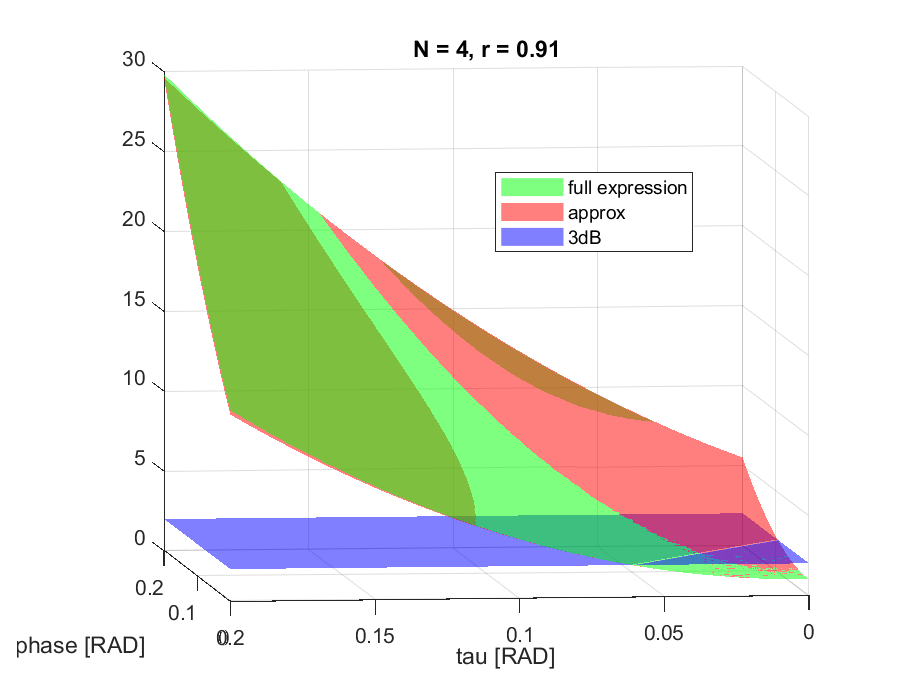
\includegraphics[width=0.9\linewidth]{./Media/spatial_IIR_MATLAB/beamwidth/BW_approx_validation.eps}
        \caption{Graphically comparing (\ref{eqn_arrayPerformance_beamwidth_fullEpxr}) and (\ref{eqn_arrayPerformance_beamwidth_approx}) for $N=4$ and $\rho=0.91$. The approximation seems to closely match the original expression.}
    \end{figure}
    Unlike the passive ULA case, it is evident from figure (\ref{fig_singleFreqFeedback_2ndTaylorNumericalValidation}) that the $4^{th}$ order terms are not needed for the evaluation of $\theta_{HPBW}$. In perfect phase alignment (i.e. $\Delta_{\tau}=0$), the u-space expression for the HPBW is $$u_{HPBW} =
    \frac{
    \left|1-\rho\right|
    }{
    \pi{d}
    }
    \lambda
    \sqrt{\frac{
    12
    }{
    \left(N-1\right)\left(\left(1+2r\right)N-4r+1\right)
    }}.
    $$
    Comparing to the classic ULA beamwidth \cite{VanTrees2002DetectionIV}, thoroughly discussed in appendix \ref{appendix_theULABeamwidth}, we can express the improvement factor as
    $$
    \frac{
    0.89\frac{\lambda}{ND}
    }{
    \theta_{HPBW,IIR}
    }
    =
    \frac{0.89}{\left|1-\rho\right|}\sqrt{\frac{1+2r}{12}}
    $$
    \todo{TODO}
    \textbf{Add graph of the improvement factor}
\fi
% \subsection{The pole-based design approach}
% In this approach, we look for setting the response "poles" which minimize the denominator, thus maximizing the overall response magnitude. To evaluate the beamwidth, we chose to allocate all of the system's poles in a single position such that 
% $
% 1-\vecnot{\beta}^{T}\vecnot{d}_{\theta}e^{-j\tau}
% =
% \left(e^{j\theta}-re^{j\theta_{s}}\right)^{N}
% $
% where $N$ is the number of array sensors and $r \in \left[0,1\right)$ enables us to avoid treatment of $\infty$-valued expressions. Next, we look for $\theta$ such that
% $
% \left|\frac{
% \frac
% {
% \vecnot{\alpha}^{T}\vecnot{d}_{\theta_{s}}
% }{
% \vecnot{\beta}^{T}\vecnot{d}_{\theta_{s}}
% }
% }{
% \frac
% {
% \vecnot{\alpha}^{T}\vecnot{d}_{\theta}
% }{
% \vecnot{\beta}^{T}\vecnot{d}_{\theta}
% }
% }\right|
% = \frac{1}{\sqrt{2}}
% $. Assuming that, like in classical IIR filter design theory, the numerator behaviour is significantly "slower" than the denominator's which results in $\vecnot{\alpha}^{T}\vecnot{d}_{\theta} 
% \approx
% \vecnot{\alpha}^{T}\vecnot{d}_{\theta_{s}}$ reults in
% \begin{align*}
%     \left|\frac{
%     \vecnot{\beta}^{T}\vecnot{d}_{\theta}
%     }{
%     \vecnot{\beta}^{T}\vecnot{d}_{\theta_{s}}
%     }\right|
%     &= \frac{1}{\sqrt{2}}
%     \\
%     \left|
%     \frac{
%     \left(e^{j\theta}-re^{j\theta}\right)^{N}
%     }{
%     \left(e^{j\theta}-re^{j\theta_{s}}\right)^{N}
%     }
%     \right|
%     &=
%     \left|
%     \frac{
%     \left(1-re^{j\left(\theta_{s}-\theta\right)}\right)
%     }{
%     \left(1-r\right)
%     }
%     \right|^{N}
%     \\
%     &=
%     \left|
%     \frac{
%     1+r^{2}-2r\cos{\left(\theta_{s}-\theta\right)}
%     }{
%     \left(1-r\right)^{2}
%     }
%     \right|^{\frac{N}{2}}
%     =
%     \left(\frac{1}{2}\right)^{\frac{1}{2}}
%     \\
%     \Rightarrow 
%     1+r^{2}-2r\cos{\left(\theta_{s}-\theta\right)}
%     &=
%     \left(1-r\right)^{2}2^{\frac{1}{N}}
%     \\
%     \cos{\left(\theta_{s}-\theta\right)}
%     &=
%     \frac{
%     1+r^{2}-\left(1-r\right)^{2}2^{\frac{1}{N}}
%     }{
%     2r
%     }
%     \\
%     \Rightarrow
%     \frac{\omega{D\left(cos(\theta_{g,s})-cos(\theta_{g,B})\right)}}{c}
%     &=
%     cos^{-1}
%     \left(
%     \frac{1+r^{2}-\left(1-r\right)^{2}2^{\frac{1}{N}}}{2r}
%     \right)
% \end{align*}.
% Therefore,
% \begin{equation}
%     \theta_{g,B} 
%     &= 
%     cos^{-1}
%     \left(
%     cos(\theta_{g,s})
%     -
%     \frac{c}{\omega{D}}
%     cos^{-1}
%     \left(
%     \frac{1+r^{2}-\left(1-r\right)^{2}2^{\frac{1}{N}}}{2r}
%     \right)
%     \right)
% \end{equation}
% Few observations can be derived from the $ \theta_{g,B} $:
% \begin{itemize}
%     \item $r\rightarrow{1}$ (i.e. setting the pole on the unit circle) causes $\theta_{g,B}\rightarrow\theta_{g,s}$ due to the $\infty$ valued response at $\theta_{g,s}$
%     \item The interval 
%     $
%     \left\{
%     \theta_{g,s}
%     \ \Bigg{|}\ 
%     cos(\theta_{g,s})
%     -
%     \frac{c}{\omega{D}}
%     cos^{-1}
%     \left(
%     \frac{1+r^{2}-\left(1-r\right)^{2}2^{\frac{1}{N}}}{2r}
%     \right)
%     <-1
%     \right\}
%     $, has no solution. In simulations, when evaluating such $\theta_{g,s}$ values, one can observe that the actual beampattern does not resemble the designed one due to the ULA geometric properties.
%     \item The number of sensors $N$ seems to have low impact on the beamwidth.
% \end{itemize}